\section{Elaborazione statistico-probabilistica delle pioggie intense della stazione di riferimento per il bacino in esame (analisi degli afflussi)}
In questo capitolo della relazione si condurrà un'analisi statistico-probabilistica degli eventi pluviometrici del bacino. In particolare, si utilizzerà la distribuzione di probabilità dei valori estremi (legge di Gumbel).\\
Successivamente, verrà effettuata la verifica dell'adattamento della serie di valori pluviometrici alla distribuzione, facendo ricorso al test di Matalas.\\
Infine, si svolgeranno i calcoli per determinare la Linea Segnalatrice di Possibilità Pluviometrica (LSPP).\\
Essendo che si andrà a svolgere i calcoli considerando solamente i massimi annuali di precipitazione, occorre che tali valori debbano: 
\begin{itemize}
    \item essere relativi ad un certo periodo di tempo (almeno 30 anni);
    \item essere \textit{casuali, omogenei, indipendenti e stazionari}.
\end{itemize} 
In particolare, essendo la procedura di calcolo uguale per ogni serie numerica, verrà svolta la spiegazione per la durata pluviometrica di 30 minuti, per poi riportare solamente i risultati.

\subsection{Verifica preliminare visiva  (mediante \textit{Plotting position} e distribuzione delle classi)}
\label{sec_plotting_position}
Prima di svolgere l'adattamento della serie pluviometrica misurata a quella degli estremi di Gumbel, occorre valutare se tali valori si adattano correttamente lungo la retta di distribuzione teorica.\\
Ad ogni misura della serie, posta in ordine crescente, viene attribuito un valore a seconda della propria posizione nel campione, secondo il metodo di Weibull $(P_{em}= \frac{i}{N+1})$ o Hazen $\left(P_{em}=\frac{i-0.5}{N}\right)$. Entrambi questi parametri correlano l'evento di precipitazione con la probabilità di non superamento dell'evento (anche indicato come $P$).\\
Utilizzando il valore ricavato da uno di questi metodi, viene calcolata una variabile d'appoggio ($y$), secondo la formula $y = -ln(-ln(P))$, essendo che $P(x)= e ^{-e^ {-y}}$.\\
\noindent Successivamente, utilizzando i parametri $y$ (appena calcolato), $\alpha$ e $u$, quest'ultimi basati sul campione, si riesce a ricavare l'altezza di precipitazione dell'evento, regolarizzata secondo la distribuzione di Gumbel, secondo la formula inversa di $y = \alpha (h - u)$.
\begin{equation}
    \alpha = \left(\frac{1.283}{\sigma(h)}\right)
\end{equation}
\begin{equation}
    u = \left( h_m - \frac{0.5772}{\alpha} \right)
\end{equation}
\begin{equation}
    h = \frac{y}{\alpha}+u
    \label{h_tr}
\end{equation}
Al fine di verificare visivamente la bontà degli allineamenti delle distribuzioni della serie osservata e della serie attesa (teorica), occorre creare un grafico dove, in ascissa si pone il valore del parametro $y$ ed in ordinata si pongono i valori delle relative precipitazioni teoriche. I grafici sono riportati nel successivo capitoletto.\\
Maggiore è l'allineamento tra le due distribuzioni e migliore sarà la distribuzione della serie osservata.\\
Inoltre, per valutare preliminarmente la serie, può essere utile suddividere le precipitazioni per classi omogenee (per vedere come si distribuiscono i valori all'interno di esse) e calcolare i principali parametri statistici.

\begin{table}[H] \centering
    \caption{\textcolor{red}{Valori di probabilità di non superamento dell'evento (calcolata mediante Weibull e Hazen) e relativo valore del parametro d'appoggio $y$, riferito ad una durata di precipitazione di 0.5 ore.}}
    \begin{tabular}{cccccc}
 &  & \multicolumn{2}{c}{\textbf{Plotting Position}} & \multicolumn{2}{c}{\textbf{Y -ln( -ln (1- 1/Tr))}}\\
 \toprule
    \textbf{n} & \textbf{h [mm] 0.5 ore} & \textbf{P Weibull   n/N+1} & \textbf{P Hazen  (n-0,5)/N} & \textbf{y Weibull} & \textbf{y Hazen}\\
\midrule
    1          & 11.2                        & 0.026                      & 0.014                       & -1.291                  & -1.460                  \\
    2          & 12                          & 0.053                      & 0.041                       & -1.080                  & -1.165                  \\
    3          & 12.2                        & 0.079                      & 0.068                       & -0.932                  & -0.991                  \\
    4          & 12.6                        & 0.105                      & 0.095                       & -0.812                  & -0.858                  \\
    5          & 13.8                        & 0.132                      & 0.122                       & -0.707                  & -0.745                  \\
    6          & 14.2                        & 0.158                      & 0.149                       & -0.613                  & -0.645                  \\
    7          & 15                          & 0.184                      & 0.176                       & -0.526                  & -0.553                  \\
    8          & 16                          & 0.211                      & 0.203                       & -0.443                  & -0.468                  \\
    9          & 16.4                        & 0.237                      & 0.230                       & -0.365                  & -0.386                  \\
    10         & 16.6                        & 0.263                      & 0.257                       & -0.289                  & -0.307                  \\
    11         & 17.2                        & 0.289                      & 0.284                       & -0.215                  & -0.231                  \\
    12         & 17.4                        & 0.316                      & 0.311                       & -0.142                  & -0.156                  \\
    13         & 17.4                        & 0.342                      & 0.338                       & -0.070                  & -0.082                  \\
    14         & 18                          & 0.368                      & 0.365                       & 0.001                   & -0.008                  \\
    15         & 18                          & 0.395                      & 0.392                       & 0.073                   & 0.065                   \\
    16         & 18.6                        & 0.421                      & 0.419                       & 0.145                   & 0.139                   \\
    17         & 19                          & 0.447                      & 0.446                       & 0.218                   & 0.214                   \\
    18         & 19.6                        & 0.474                      & 0.473                       & 0.291                   & 0.289                   \\
    19         & 20                          & 0.500                      & 0.500                       & 0.367                   & 0.367                   \\
    20         & 20.2                        & 0.526                      & 0.527                       & 0.443                   & 0.446                   \\
    21         & 20.4                        & 0.553                      & 0.554                       & 0.522                   & 0.527                   \\
    22         & 21                          & 0.579                      & 0.581                       & 0.604                   & 0.611                   \\
    23         & 22.4                        & 0.605                      & 0.608                       & 0.689                   & 0.698                   \\
    24         & 22.6                        & 0.632                      & 0.635                       & 0.778                   & 0.790                   \\
    25         & 22.6                        & 0.658                      & 0.662                       & 0.871                   & 0.886                   \\
    26         & 23.4                        & 0.684                      & 0.689                       & 0.969                   & 0.988                   \\
    27         & 25.6                        & 0.711                      & 0.716                       & 1.074                   & 1.097                   \\
    28         & 25.6                        & 0.737                      & 0.743                       & 1.186                   & 1.215                   \\
    29         & 25.8                        & 0.763                      & 0.770                       & 1.308                   & 1.343                   \\
    30         & 26.6                        & 0.789                      & 0.797                       & 1.442                   & 1.485                   \\
    31         & 27                          & 0.816                      & 0.824                       & 1.592                   & 1.644                   \\
    32         & 27                          & 0.842                      & 0.851                       & 1.761                   & 1.827                   \\
    33         & 27.8                        & 0.868                      & 0.878                       & 1.958                   & 2.043                   \\
    34         & 27.8                        & 0.895                      & 0.905                       & 2.196                   & 2.309                   \\
    35         & 29.4                        & 0.921                      & 0.932                       & 2.498                   & 2.660                   \\
    36         & 32.6                        & 0.947                      & 0.959                       & 2.918                   & 3.185                   \\
    37         & 38.4                        & 0.974                      & 0.986                       & 3.624                   & 4.297         \\
    \bottomrule         
    \end{tabular}
    \end{table}

\begin{table}[H] \centering
    \caption{\textcolor{red}{Principali parametri statistici riferiti alla serie pluviometrica di durata 0.5 ore.}}
 \begin{tabular}{cc}
    \toprule
deviazione standard ($\sigma$) & 6.2  \\
media ($x_m$)              & 20.8 \\
$\alpha$            & 0.2  \\
$u$           & 18.1\\
N                & 37.0 \\
minimo ($x_{min}$)             & 11.2 \\
massimo ($x_{max}$)            & 38.4 \\
varianza ($\sigma^2$)             & 38.3 \\
coeff. variazione (CV)    & 0.30 \\
mediana ($x_{mediana}$)        & 20.0 \\
numero di classi (k)      & 5.5  \\
k scelto                 & 6.0  \\
verifica (Iman e Canover) & 64.0 \\
delta classe ($\Delta$)          & 4.5  \\
delta scelto             & 5.0 \\
        \bottomrule
        \end{tabular}
\end{table}    

\begin{figure}[H]\centering
    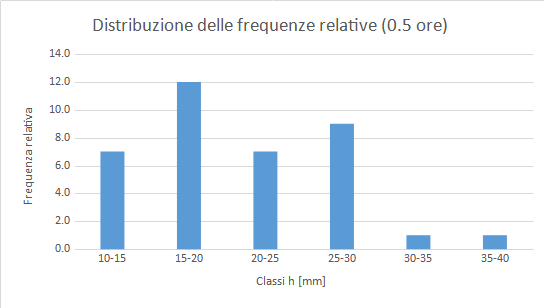
\includegraphics[scale=.6]{immagini/freq_piogg_rel_05ore.png}
    \caption{Frequenze di pioggia relativa (suddivise per classi omogenee), relative ad un evento di durata 0.5 ore.}
  \label{freq_rel_piogg_05ore}
\end{figure}

\begin{figure}[H]\centering
    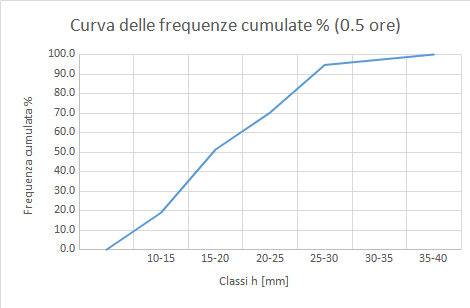
\includegraphics[scale=.6]{immagini/freq_piogg_cum_05ore.png}
    \caption{Frequenze di pioggia cumulata, relative ad un evento di durata 0.5 ore.}
  \label{freq_cum_piogg_05ore}
\end{figure}

\subsection{Calcolo delle altezze di pioggia per il $T_r$ di riferimento}
Successivamente ad aver verificato che l'allineamento tra le due distribuzioni sia apprezzabile, occorre svolgere il calcolo delle altezze di pioggia, dati dei tempi di ritorno.\\
Essendo che $y = -ln(-ln(P))$ e $P = 1-\frac{1}{T_r}$, allora 
\begin{equation}
y = -ln\left(-ln\left(1-\frac{1}{T_r}\right)\right)
\end{equation}
Partendo da questo calcolo della variabile d'appoggio, è possibile ricavare l'altezza di precipitazione mediante la formula \ref{h_tr}.

\begin{table}[H] \centering
    \caption{\textcolor{red}{Valori di altezza di pioggia attesa (teorica), calcolata mediante la variabile d'appoggio $y$ di Weibull o di Hazen.}}
    \begin{tabular}{cccc}
 & & \multicolumn{2}{c}{$h = Y/\alpha + u$}       \\
 \toprule
    \textbf{n} & \textbf{h (mm)     0.5 ore} & \textbf{h mediante Weibull} & \textbf{h mediante Hazen} \\
\midrule
    1          & 11.2                        & 11.839                & 11.028                 \\
    2          & 12                          & 12.858                & 12.449                 \\
    3          & 12.2                        & 13.573                & 13.286                 \\
    4          & 12.6                        & 14.153                & 13.929                 \\
    5          & 13.8                        & 14.656                & 14.472                 \\
    6          & 14.2                        & 15.110                & 14.955                 \\
    7          & 15                          & 15.531                & 15.397                 \\
    8          & 16                          & 15.927                & 15.811                 \\
    9          & 16.4                        & 16.306                & 16.205                 \\
    10         & 16.6                        & 16.672                & 16.584                 \\
    11         & 17.2                        & 17.029                & 16.953                 \\
    12         & 17.4                        & 17.380                & 17.314                 \\
    13         & 17.4                        & 17.727                & 17.671                 \\
    14         & 18                          & 18.073                & 18.026                 \\
    15         & 18                          & 18.418                & 18.380                 \\
    16         & 18.6                        & 18.765                & 18.737                 \\
    17         & 19                          & 19.115                & 19.096                 \\
    18         & 19.6                        & 19.471                & 19.461                 \\
    19         & 20                          & 19.833                & 19.833                 \\
    20         & 20.2                        & 20.203                & 20.214                 \\
    21         & 20.4                        & 20.585                & 20.606                 \\
    22         & 21                          & 20.979                & 21.011                 \\
    23         & 22.4                        & 21.388                & 21.433                 \\
    24         & 22.6                        & 21.815                & 21.874                 \\
    25         & 22.6                        & 22.263                & 22.338                 \\
    26         & 23.4                        & 22.738                & 22.831                 \\
    27         & 25.6                        & 23.243                & 23.356                 \\
    28         & 25.6                        & 23.785                & 23.924                 \\
    29         & 25.8                        & 24.374                & 24.542                 \\
    30         & 26.6                        & 25.020                & 25.225                 \\
    31         & 27                          & 25.740                & 25.993                 \\
    32         & 27                          & 26.557                & 26.874                 \\
    33         & 27.8                        & 27.509                & 27.915                 \\
    34         & 27.8                        & 28.655                & 29.199                 \\
    35         & 29.4                        & 30.111                & 30.891                 \\
    36         & 32.6                        & 32.133                & 33.422                 \\
    37         & 38.4                        & 35.541                & 38.786          \\
    \bottomrule      
    \end{tabular}
    \end{table}

    \begin{figure}[H]\centering
        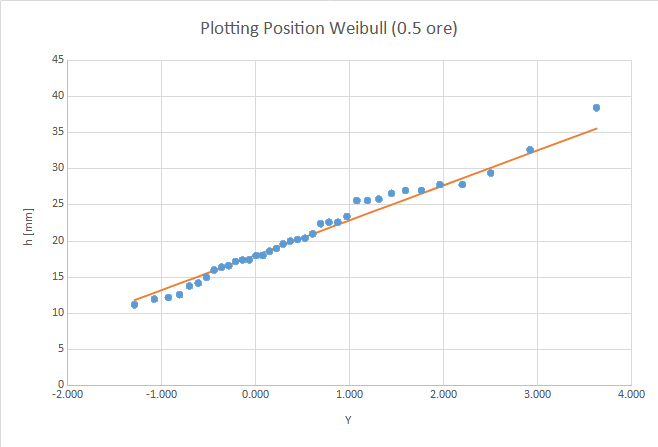
\includegraphics[scale=.5]{immagini/plot_pos_weib_05ore.png}
        \caption{Plotting position mediante weibull.}
      \label{plot_pos_weib_05ore}
    \end{figure}

    \begin{figure}[H]\centering
        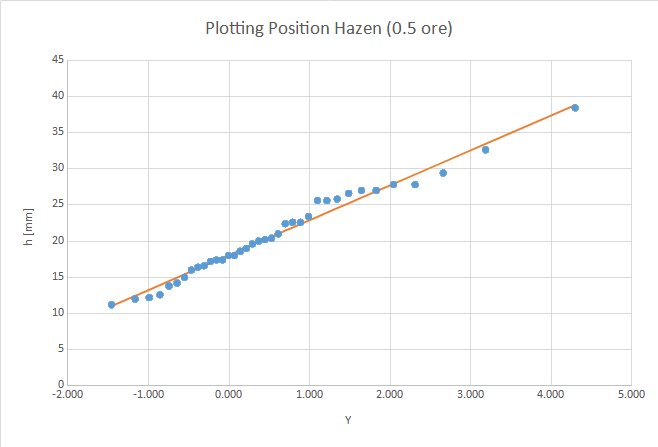
\includegraphics[scale=.5]{immagini/plot_pos_hazen_05ore.png}
        \caption{Plottin position mediante Hazen.}
      \label{plot_pos_hazen_05ore}
    \end{figure}

\begin{table}[H] \centering
        \begin{tabular}{ccc}
        \toprule
        Tr (anni) & y     & h attesa (mm) \\
        \midrule
        2 & 0.367 & 19.8  \\
        5 & 1.500 & 25.3  \\
        10  & 2.250 & 28.9          \\
        30  & 3.384 & 34.4          \\
        50  & 3.902 & 36.9          \\
        100 & 4.600 & 40.2          \\
        200 & 5.296 & 43.6          \\         
        \bottomrule
        \end{tabular}
\end{table}
    
\subsection{Test statistico di Matalas}
Similmente a come è stata svolta la verifica grafica (\ref{sec_plotting_position}), è necessario accertarsi che l'asimmetria ($G$) della serie osservata (storica) non differisca eccessivamente dalla serie teorica.\\
La procedura del test statistico è:
\begin{itemize}
\item calcolo del coefficiente di asimmetria $G$, mediante \ref{coef_asimmetria};
\item estrapolazione dei parametri $E(y)$ e $\sigma(y)$, in funzione di N;
\item verifica della disequazione \ref{disequazione_matalas}.
\end{itemize}
\begin{equation}
    G = \frac{m_3}{m_2^{\frac{3}{2}}} = N^{\frac{1}{2}} \frac{\sum_{i=1,N}(x_i - x_m)^3}{\left[\sum_{i=1,N}(x_i-x_m)^2\right]^{\frac{3}{2}}}
    \label{coef_asimmetria}
\end{equation}
\begin{equation}
    |G - E (y)| < 2 \sigma(y)
    \label{disequazione_matalas}
\end{equation}
\noindent Dove:
\begin{itemize}
    \item $G$: coefficiente di asimmetria del campione;
    \item $E(y)$: coefficiente di asimmetria del campione perfetto, che segue l'andamento di Gumbel;
    \item $\sigma (y)$: deviazione standard del campione.
\end{itemize}
Nel caso in cui la disequazione fosse corretta, è possibile accettare la distribuzione di probabilità di Gumbel. In caso contrario occorrerebbe provare un'altra distribuzione teorica di probabilità.

\begin{table}[H] \centering
    \caption{\textcolor{red}{Parametri per l'esecuzione del test statistico di Matalas, relativi alla durata di precipitazione di 0.5 ore.}}
    \begin{tabular}{cc}
    \toprule
    media                  & 20.85 \\
    $N ^{0.5}$ & 6.083 \\
    G                      & 0.622 \\
    G - E                  & 0.259 \\
    2 $\sigma$             & 1.069 \\
    TEST                   & Vero \\
    \bottomrule
    \end{tabular}
\end{table}

\subsection{Risultati delle altre durate di precipitazione}
Come anticipato precedentemente, in questa sezione vengono riportati solamente i risultati delle analisi matematiche (tabelle e grafici) per le altre durate di precipitazione.\\
I procedimenti per le seguenti durate sono i medesimi utilizzati per la durata di 0.5 ore.
\subsubsection{Durata di 1 ora}
\begin{table}[H] \centering
    \begin{tabular}{cccccc}
        &  & \multicolumn{2}{c}{\textbf{Plotting Position}} & \multicolumn{2}{c}{\textbf{Y -ln( -ln (1- 1/Tr))}}\\
        \toprule
           \textbf{n} & \textbf{h [mm] 1 ora} & \textbf{P Weibull   n/N+1} & \textbf{P Hazen  (n-0,5)/N} & \textbf{y Weibull} & \textbf{y Hazen}\\
       \midrule
    1          & 13.8                      & 0.026                      & 0.014                       & -1.291                  & -1.460                  \\
    2          & 14.4                      & 0.053                      & 0.041                       & -1.080                  & -1.165                  \\
    3          & 16.2                      & 0.079                      & 0.068                       & -0.932                  & -0.991                  \\
    4          & 17                        & 0.105                      & 0.095                       & -0.812                  & -0.858                  \\
    5          & 17.6                      & 0.132                      & 0.122                       & -0.707                  & -0.745                  \\
    6          & 17.8                      & 0.158                      & 0.149                       & -0.613                  & -0.645                  \\
    7          & 19.2                      & 0.184                      & 0.176                       & -0.526                  & -0.553                  \\
    8          & 19.4                      & 0.211                      & 0.203                       & -0.443                  & -0.468                  \\
    9          & 19.4                      & 0.237                      & 0.230                       & -0.365                  & -0.386                  \\
    10         & 20.6                      & 0.263                      & 0.257                       & -0.289                  & -0.307                  \\
    11         & 20.6                      & 0.289                      & 0.284                       & -0.215                  & -0.231                  \\
    12         & 21.2                      & 0.316                      & 0.311                       & -0.142                  & -0.156                  \\
    13         & 21.6                      & 0.342                      & 0.338                       & -0.070                  & -0.082                  \\
    14         & 21.8                      & 0.368                      & 0.365                       & 0.001                   & -0.008                  \\
    15         & 23.6                      & 0.395                      & 0.392                       & 0.073                   & 0.065                   \\
    16         & 23.6                      & 0.421                      & 0.419                       & 0.145                   & 0.139                   \\
    17         & 23.8                      & 0.447                      & 0.446                       & 0.218                   & 0.214                   \\
    18         & 24                        & 0.474                      & 0.473                       & 0.291                   & 0.289                   \\
    19         & 24.2                      & 0.500                      & 0.500                       & 0.367                   & 0.367                   \\
    20         & 24.4                      & 0.526                      & 0.527                       & 0.443                   & 0.446                   \\
    21         & 24.4                      & 0.553                      & 0.554                       & 0.522                   & 0.527                   \\
    22         & 24.8                      & 0.579                      & 0.581                       & 0.604                   & 0.611                   \\
    23         & 25.8                      & 0.605                      & 0.608                       & 0.689                   & 0.698                   \\
    24         & 26.8                      & 0.632                      & 0.635                       & 0.778                   & 0.790                   \\
    25         & 27                        & 0.658                      & 0.662                       & 0.871                   & 0.886                   \\
    26         & 27.6                      & 0.684                      & 0.689                       & 0.969                   & 0.988                   \\
    27         & 28                        & 0.711                      & 0.716                       & 1.074                   & 1.097                   \\
    28         & 28.8                      & 0.737                      & 0.743                       & 1.186                   & 1.215                   \\
    29         & 30.2                      & 0.763                      & 0.770                       & 1.308                   & 1.343                   \\
    30         & 30.2                      & 0.789                      & 0.797                       & 1.442                   & 1.485                   \\
    31         & 30.4                      & 0.816                      & 0.824                       & 1.592                   & 1.644                   \\
    32         & 31.2                      & 0.842                      & 0.851                       & 1.761                   & 1.827                   \\
    33         & 31.6                      & 0.868                      & 0.878                       & 1.958                   & 2.043                   \\
    34         & 34.2                      & 0.895                      & 0.905                       & 2.196                   & 2.309                   \\
    35         & 37.8                      & 0.921                      & 0.932                       & 2.498                   & 2.660                   \\
    36         & 42.6                      & 0.947                      & 0.959                       & 2.918                   & 3.185                   \\
    37         & 49.8                      & 0.974                      & 0.986                       & 3.624                   & 4.297        \\
    \bottomrule          
    \end{tabular}
    \end{table}

\subsubsection{Durata di 3 ore}
\begin{table}[H] \centering
\begin{tabular}{cccccc}
    &  & \multicolumn{2}{c}{\textbf{Plotting Position}} & \multicolumn{2}{c}{\textbf{Y -ln( -ln (1- 1/Tr))}}\\
    \toprule
       \textbf{n} & \textbf{h [mm] 1 ora} & \textbf{P Weibull   n/N+1} & \textbf{P Hazen  (n-0,5)/N} & \textbf{y Weibull} & \textbf{y Hazen}\\
   \midrule 
    1          & 18.6                      & 0.026                      & 0.014                       & -1.291                  & -1.460                  \\
    2          & 19.6                      & 0.053                      & 0.041                       & -1.080                  & -1.165                  \\
    3          & 21.8                      & 0.079                      & 0.068                       & -0.932                  & -0.991                  \\
    4          & 21.8                      & 0.105                      & 0.095                       & -0.812                  & -0.858                  \\
    5          & 23.4                      & 0.132                      & 0.122                       & -0.707                  & -0.745                  \\
    6          & 24.6                      & 0.158                      & 0.149                       & -0.613                  & -0.645                  \\
    7          & 24.8                      & 0.184                      & 0.176                       & -0.526                  & -0.553                  \\
    8          & 25.4                      & 0.211                      & 0.203                       & -0.443                  & -0.468                  \\
    9          & 26.8                      & 0.237                      & 0.230                       & -0.365                  & -0.386                  \\
    10         & 27.8                      & 0.263                      & 0.257                       & -0.289                  & -0.307                  \\
    11         & 28                        & 0.289                      & 0.284                       & -0.215                  & -0.231                  \\
    12         & 30.4                      & 0.316                      & 0.311                       & -0.142                  & -0.156                  \\
    13         & 30.4                      & 0.342                      & 0.338                       & -0.070                  & -0.082                  \\
    14         & 31.2                      & 0.368                      & 0.365                       & 0.001                   & -0.008                  \\
    15         & 31.8                      & 0.395                      & 0.392                       & 0.073                   & 0.065                   \\
    16         & 32.8                      & 0.421                      & 0.419                       & 0.145                   & 0.139                   \\
    17         & 33                        & 0.447                      & 0.446                       & 0.218                   & 0.214                   \\
    18         & 33.2                      & 0.474                      & 0.473                       & 0.291                   & 0.289                   \\
    19         & 33.2                      & 0.500                      & 0.500                       & 0.367                   & 0.367                   \\
    20         & 33.8                      & 0.526                      & 0.527                       & 0.443                   & 0.446                   \\
    21         & 34                        & 0.553                      & 0.554                       & 0.522                   & 0.527                   \\
    22         & 35.4                      & 0.579                      & 0.581                       & 0.604                   & 0.611                   \\
    23         & 35.8                      & 0.605                      & 0.608                       & 0.689                   & 0.698                   \\
    24         & 35.8                      & 0.632                      & 0.635                       & 0.778                   & 0.790                   \\
    25         & 35.8                      & 0.658                      & 0.662                       & 0.871                   & 0.886                   \\
    26         & 36                        & 0.684                      & 0.689                       & 0.969                   & 0.988                   \\
    27         & 36.2                      & 0.711                      & 0.716                       & 1.074                   & 1.097                   \\
    28         & 37.2                      & 0.737                      & 0.743                       & 1.186                   & 1.215                   \\
    29         & 38.2                      & 0.763                      & 0.770                       & 1.308                   & 1.343                   \\
    30         & 38.4                      & 0.789                      & 0.797                       & 1.442                   & 1.485                   \\
    31         & 41.4                      & 0.816                      & 0.824                       & 1.592                   & 1.644                   \\
    32         & 41.6                      & 0.842                      & 0.851                       & 1.761                   & 1.827                   \\
    33         & 44.8                      & 0.868                      & 0.878                       & 1.958                   & 2.043                   \\
    34         & 45.8                      & 0.895                      & 0.905                       & 2.196                   & 2.309                   \\
    35         & 46                        & 0.921                      & 0.932                       & 2.498                   & 2.660                   \\
    36         & 50.6                      & 0.947                      & 0.959                       & 2.918                   & 3.185                   \\
    37         & 75.4                      & 0.974                      & 0.986                       & 3.624                   & 4.297              \\
    \bottomrule    
    \end{tabular}
    \end{table}

\subsubsection{Durata di 6 ore}
\begin{table}[H] \centering
    \begin{tabular}{cccccc}
        &  & \multicolumn{2}{c}{\textbf{Plotting Position}} & \multicolumn{2}{c}{\textbf{Y -ln( -ln (1- 1/Tr))}}\\
        \toprule
           \textbf{n} & \textbf{h [mm] 1 ora} & \textbf{P Weibull   n/N+1} & \textbf{P Hazen  (n-0,5)/N} & \textbf{y Weibull} & \textbf{y Hazen}\\
       \midrule 
    1          & 25                          & 0.026                      & 0.014                       & -1.291                  & -1.460                  \\
    2          & 26.4                        & 0.053                      & 0.041                       & -1.080                  & -1.165                  \\
    3          & 26.8                        & 0.079                      & 0.068                       & -0.932                  & -0.991                  \\
    4          & 27.8                        & 0.105                      & 0.095                       & -0.812                  & -0.858                  \\
    5          & 30.4                        & 0.132                      & 0.122                       & -0.707                  & -0.745                  \\
    6          & 32.6                        & 0.158                      & 0.149                       & -0.613                  & -0.645                  \\
    7          & 32.8                        & 0.184                      & 0.176                       & -0.526                  & -0.553                  \\
    8          & 33                          & 0.211                      & 0.203                       & -0.443                  & -0.468                  \\
    9          & 33.6                        & 0.237                      & 0.230                       & -0.365                  & -0.386                  \\
    10         & 35.6                        & 0.263                      & 0.257                       & -0.289                  & -0.307                  \\
    11         & 37.2                        & 0.289                      & 0.284                       & -0.215                  & -0.231                  \\
    12         & 37.6                        & 0.316                      & 0.311                       & -0.142                  & -0.156                  \\
    13         & 37.8                        & 0.342                      & 0.338                       & -0.070                  & -0.082                  \\
    14         & 38.4                        & 0.368                      & 0.365                       & 0.001                   & -0.008                  \\
    15         & 39.4                        & 0.395                      & 0.392                       & 0.073                   & 0.065                   \\
    16         & 41.8                        & 0.421                      & 0.419                       & 0.145                   & 0.139                   \\
    17         & 41.8                        & 0.447                      & 0.446                       & 0.218                   & 0.214                   \\
    18         & 42.2                        & 0.474                      & 0.473                       & 0.291                   & 0.289                   \\
    19         & 42.6                        & 0.500                      & 0.500                       & 0.367                   & 0.367                   \\
    20         & 44.4                        & 0.526                      & 0.527                       & 0.443                   & 0.446                   \\
    21         & 44.8                        & 0.553                      & 0.554                       & 0.522                   & 0.527                   \\
    22         & 45                          & 0.579                      & 0.581                       & 0.604                   & 0.611                   \\
    23         & 46.6                        & 0.605                      & 0.608                       & 0.689                   & 0.698                   \\
    24         & 47.2                        & 0.632                      & 0.635                       & 0.778                   & 0.790                   \\
    25         & 48                          & 0.658                      & 0.662                       & 0.871                   & 0.886                   \\
    26         & 48.8                        & 0.684                      & 0.689                       & 0.969                   & 0.988                   \\
    27         & 50.6                        & 0.711                      & 0.716                       & 1.074                   & 1.097                   \\
    28         & 51.4                        & 0.737                      & 0.743                       & 1.186                   & 1.215                   \\
    29         & 51.4                        & 0.763                      & 0.770                       & 1.308                   & 1.343                   \\
    30         & 51.8                        & 0.789                      & 0.797                       & 1.442                   & 1.485                   \\
    31         & 52.8                        & 0.816                      & 0.824                       & 1.592                   & 1.644                   \\
    32         & 53.2                        & 0.842                      & 0.851                       & 1.761                   & 1.827                   \\
    33         & 55.6                        & 0.868                      & 0.878                       & 1.958                   & 2.043                   \\
    34         & 58.2                        & 0.895                      & 0.905                       & 2.196                   & 2.309                   \\
    35         & 65.4                        & 0.921                      & 0.932                       & 2.498                   & 2.660                   \\
    36         & 71.6                        & 0.947                      & 0.959                       & 2.918                   & 3.185                   \\
    37         & 130.2                       & 0.974                      & 0.986                       & 3.624                   & 4.297                  
    \end{tabular}
    \end{table}

\subsection{LSPP - Linee segnalatrici di probabilità pluviometrica}
Dopo aver ottenuto le quantità di precipitazioni teoriche, per ogni durata di evento pluviometrico e per diversi tempi di ritorno, è possibile creare un grafico che metta in relazione tutti questi parametri.\\
La curva risultate ha un andamento caratteristico che segue la funzione $h=at^n$, con $a$ che dipende dal tempo di ritorno T e con $n$ che risulta essere una costante per la stazione di rilevamento dei dati (in Italia generalmente è tra 0.20 e 0.55). Il parametro $n$ ha un valore sempre inferiore ad 1 perchè all'aumentare del tempo dell'evento pluviometrico, l'intensità di pioggia cala.\\
Nel caso in cui gli assi del grafico avessero entrambi la scala logaritmica, la linea interpolatrice dei punti sarebbe una retta.


